\documentclass[CJK,notheorems,compress,mathserif,table]{beamer}
\usepackage{ifxetex}
\usepackage{ifpdf}

%\useoutertheme[height=0.1\textwidth,width=0.15\textwidth,hideothersubsections]{sidebar}
%\usecolortheme{whale}      % Outer color themes: whale, seahorse, dolphin
%\usecolortheme{orchid}     % Inner color themes: lily, orchid
%\useinnertheme[shadow]{rounded}
%\setbeamercolor{sidebar}{bg=blue!50}
%\setbeamercolor{background canvas}{bg=blue!9}
%\usefonttheme{serif}
\setbeamertemplate{navigation symbols}{}
\usetheme{default}

%%------------------------常用宏包---------------------------------------------------------------------

\mode<article> % 仅应用于article版本
{
  \usepackage{beamerbasearticle}
  \usepackage{fullpage}
  \usepackage{hyperref}
}
%\usepackage[font=Times, timeinterval=10, timeduration=30,
%timewarningfirst=85, timewarningsecond=90,
%fillcolorwarningsecond=white!60!yellow]{tdclock}
%\setbeameroption{show notes}
\setbeameroption{hide notes}
%\usepackage{ifpdf}
%% 下面的包控制beamer的风格,可以根据自己的爱好修改
\usepackage{beamerthemesplit}   % 使用split风格
\usepackage{beamerthemeshadow}  % 使用shadow风格
\usepackage{amsmath,amssymb}
\ifxetex
  \usepackage[BoldFont,SlantFont,CJKchecksingle]{xeCJK}
  \setCJKmainfont[BoldFont=SimHei]{SimSun}
  \setCJKmonofont{SimSun}% 设置缺省中文字体

%  \DeclareGraphicsExtensions{.pdf,.jpg,.jpeg,.png}
\else
  \usepackage{CJKutf8}
  \usepackage{CJKnumb}
  \usepackage{CJKpunct}
  \usepackage{CJKspace}
%	\ifpdf
%	  \usepackage[pdftex]{graphicx}
%	  \graphicspath{./pics/}
%	  \DeclareGraphicsExtensions{.pdf,.jpeg,.png}
%	\else
%	  \usepackage[dvips]{graphicx}
%	  \graphicspath{{./pics/}}
%	  \DeclareGraphicsExtensions{.eps,.ps}
%	\fi
\fi
\usepackage{graphicx}
\graphicspath{{./pics/}}

%\usepackage{CJKutf8}
\usepackage{hyperref}
\hypersetup{CJKbookmarks=true}
%\usepackage{graphicx}
%\graphicspath{{./pics/}}
%%\DeclareGraphicsRule{*}{mps}{*}{}
\usepackage{subfigure}
\usepackage{xmpmulti}
\usepackage{colortbl,dcolumn}
\usepackage{multimedia}
\usepackage{chemarr}
%pgf由beamer的开发者tantau开发,由以在beamer中精确作图。
\usepackage{pgf,pgfarrows,pgfnodes,pgfautomata,pgfheaps}

%% 下面的代码用来读入Logo图象
%\pgfdeclaremask{logomask}{pics/thu-logo1-mask.eps}
%\pgfdeclareimage[mask=logomask,height=1.5cm]{logo}{pics/thu-logo1.eps}

%设置logo图标
%\logo{
\includegraphics[height=0.09\textwidth]{pics/thu-logo2.jpg}}
\logo{
\includegraphics[height=0.09\textwidth,bb=0 0 489 490]{pics/thu-logo2.png}}

\renewcommand{\raggedright}{\leftskip=0pt \rightskip=0pt plus 0cm}
\raggedright

\def\hilite<#1>{%
\temporal<#1>{\color{blue!35}}{\color{magenta}}%
{\color{blue!75}}}

\newcolumntype{H}{>{\columncolor{blue!20}}c!{\vrule}}
\newcolumntype{H}{>{\columncolor{blue!20}}c}
%==================================参考文献==============================================================
\newcommand{\upcite}[1]{\textsuperscript{\cite{#1}}}  %自定义命令\upcite, 使参考文献引用以上标出现
%\bibliographystyle{plain}% set in slidereference.tex
%%%%%%%%%%%%%%%%%%%%%%%%%%%%%%%%%%%%%%重定义字体、字号命令 %%%%%%%%%%%%%%%%%%%%%%%%%%%%%%%%%%%%%%%%%%%%%%
\newcommand{\songti}{\CJKfamily{song}}        % 宋体
\newcommand{\fangsong}{\CJKfamily{fs}}        % 仿宋体
\newcommand{\kaishu}{\CJKfamily{kai}}         % 楷体
\newcommand{\heiti}{\CJKfamily{hei}}          % 黑体
\newcommand{\lishu}{\CJKfamily{li}}           % 隶书
\newcommand{\youyuang}{\CJKfamily{you}}       % 幼圆
\newcommand{\sihao}{\fontsize{14pt}{\baselineskip}\selectfont}      % 字号设置
\newcommand{\xiaosihao}{\fontsize{12pt}{\baselineskip}\selectfont}  % 字号设置
\newcommand{\wuhao}{\fontsize{10.5pt}{\baselineskip}\selectfont}    % 字号设置
\newcommand{\xiaowuhao}{\fontsize{9pt}{\baselineskip}\selectfont}   % 字号设置
\newcommand{\liuhao}{\fontsize{7.875pt}{\baselineskip}\selectfont}  % 字号设置
\newcommand{\qihao}{\fontsize{5.25pt}{\baselineskip}\selectfont}    % 字号设置
%%%%%%%%%%%%%%%%%%%%%%%%%%%%%%%%%%%%%%%%%%%%%%%%%%%%%%%%%%%%%%%%%%%%%%%%%%%%%%%%%%%%%%%%%%%%%%%%%%%%%%%%
\newcommand{\argmax}{\operatornamewithlimits{argmax}}
\newcommand{\argmin}{\operatornamewithlimits{argmin}}
\newcommand{\tfn}[1]{\footnote{\tiny #1}}
\begin{document}
%\initclock
\ifxetex
\else
\begin{CJK}{UTF8}{song}
\fi
\ifxetex
%\pgfdeclaremask{thumask}{pics/thu-mark1-mask.png}
%\pgfdeclareimage[mask=thumask,height=0.25cm]{thu}{pics/thu-mark1.png}
\pgfdeclareimage[height=0.25cm]{thu}{pics/thu-mark1.png}
\pgfdeclareimage[height=0.25cm]{thunew}{pics/thu-mark1.png}

%\pgfdeclaremask{titlelogomask}{pics/thu-gate2-mask.jpg}
%\pgfdeclareimage[mask=titlelogomask,height=2.5cm]{titlelogo}{pics/thu-gate2.jpg}
\pgfdeclareimage[height=2.5cm]{titlelogo}{pics/thu-gate2.jpg}
\pgfdeclareimage[height=2.5cm]{titlelogonew}{pics/thu-gate2.jpg}
\else
\ifpdf
\pgfdeclaremask{thumask}{pics/thu-mark1-mask.png}
\pgfdeclareimage[mask=thumask,height=0.25cm]{thu}{pics/thu-mark1.png}
\pgfdeclareimage[height=0.4cm]{thunew}{pics/thu-mark1.png}

\pgfdeclaremask{titlelogomask}{pics/thu-gate2-mask.jpg}
\pgfdeclareimage[mask=titlelogomask,height=2.5cm]{titlelogo}{pics/thu-gate2.jpg}
\pgfdeclareimage[height=2.5cm]{titlelogonew}{pics/thu-gate2.jpg}
\else
\pgfdeclaremask{thumask}{pics/thu-mark1-mask.eps}
\pgfdeclareimage[mask=thumask,height=0.25cm]{thu}{pics/thu-mark1.eps}

\pgfdeclaremask{titlelogomask}{pics/thu-gate2-mask.eps}
\pgfdeclareimage[mask=titlelogomask,height=2.5cm]{titlelogo}{pics/thu-gate2.eps}
\fi
\fi

%  \begin{CJK*}{UTF8}{song}
%%----------------------- Theorems ---------------------------------------------------------------------
%\theoremstyle{plain} %\theoremheaderfont{\heiti}
%\theorembodyfont{\songti} \theoremindent0em
%\theoremseparator{\hspace{1em}} \theoremnumbering{arabic}
%\theoremsymbol{} %定理结束时自动添加的标志
%\newtheorem{problem}{Problem. }
\newtheorem{problem}{问题}
\newtheorem{asm}{假定}
\newtheorem{theorem}{定理}
%\newtheorem{theorem}{Theorem}
\newtheorem{definition}{定义}
%\newtheorem{definition}{Definition.}
\newtheorem{lemma}{引理}
\newtheorem{corollary}{推论}
%\newtheorem{corollary}{Corollary}
\newtheorem{proposition}{命题}
\newtheorem{example}{例}
\newtheorem{remark}{注}
\newtheorem{solution}{解答}
\newcommand\term[1]{#1}
\def\semichecked{\checkmark\!\!\!\raisebox{0.4 em}{\tiny$\smallsetminus$}}
\definecolor{Gray}{gray}{0.75}
%\renewcommand\figurename{\rm 图}
%\renewcommand\tablename{\bf 表}
\renewcommand\figurename{\rm Figure}
\renewcommand\tablename{\bf Table}

\AtBeginSection[]{ % 在每个Subsection前都会加入的Frame
  \frame<handout:0>{
    \frametitle{目录}
%\tableofcontents[current,hideallsubsections]%
\tableofcontents[sectionstyle=show/shaded,subsectionstyle=show/show/hide]%
%    \tableofcontents[currentsubsection]
%\tableofcontents[current,currentsubsection]%currentsection(或 currentsubsection) 仅正常显示当前节(小节)目录,其他部 分半透明 
  }
}
\AtBeginSubsection[]{ % 在每个Subsection前都会加入的Frame
  \frame<handout:0>{
    \frametitle{目录}
%\tableofcontents[current,hideothersubsections,currentsubsection]%
	\tableofcontents[sectionstyle=show/shaded,subsectionstyle=show/shaded/hide]
%\tableofcontents[current,currentsubsection]%
%    \tableofcontents[currentsubsection]
  }
}

\setbeamertemplate{background canvas}[vertical shading][bottom=white,top=structure.fg!25]
\ifxetex
%\titlegraphic{\pgfuseimage{titlelogonew}}
\else
\ifpdf
%\titlegraphic{\pgfuseimage{titlelogonew}}
\else
%\titlegraphic{\pgfuseimage{titlelogo}}
\fi
\fi
\makeatletter
\newcommand{\setfoot}[1]{
\usefoottemplate{ %重新定义页脚,加入作者,单位,单位图标,和文档标题
  \vbox{\tiny%
    \hbox{%
      \setbox\beamer@linebox=\hbox to\paperwidth{%
		\ifxetex
		%\hbox to.5\paperwidth{\hfill\tiny\color{white}\textbf{\insertshortauthor\quad\insertshortinstitute}\hskip.1cm\lower 0.35em\hbox{\pgfuseimage{thunew}}\hskip.3cm}%
        \hbox to.5\paperwidth{\hfill\tiny\color{white}\textbf{
		\insertpagenumber/90\quad\insertshortinstitute}\color{black}#1\hskip.0cm\lower 0.35em\hbox{\pgfuseimage{thunew}}\hskip.3cm}%
		\else
	  	\ifpdf
        \hbox to.5\paperwidth{\hfill\tiny\color{white}\textbf{\insertshortauthor\quad\insertshortinstitute}\hskip.1cm\lower 0.35em\hbox{\pgfuseimage{thunew}}\hskip.3cm}%
		\else
        \hbox to.5\paperwidth{\hfill\tiny\color{white}\textbf{\insertshortauthor\quad\insertshortinstitute}\hskip.1cm\lower 0.35em\hbox{\pgfuseimage{thu}}\hskip.3cm}%
		\fi
		\fi
        \hbox to.5\paperwidth{\hskip.3cm\tiny\color{white}\textbf{\insertshorttitle}\hfill}\hfill}%
      \ht\beamer@linebox=2.625ex%
      \dp\beamer@linebox=0pt%
      \setbox\beamer@linebox=\vbox{\box\beamer@linebox\vskip1.125ex}%
      \color{structure}\hskip-\Gm@lmargin\vrule width.5\paperwidth
      height\ht\beamer@linebox\color{structure!70}\vrule width.5\paperwidth
      height\ht\beamer@linebox\hskip-\paperwidth%
      \hbox{\box\beamer@linebox\hfill}\hfill\hskip-\Gm@rmargin}
  }
}
}
\setfoot{}
%\usefoottemplate{ %重新定义页脚,加入作者,单位,单位图标,和文档标题
%  \vbox{\tiny%
%    \hbox{%
%      \setbox\beamer@linebox=\hbox to\paperwidth{%
%		\ifxetex
%		%\hbox to.5\paperwidth{\hfill\tiny\color{white}\textbf{\insertshortauthor\quad\insertshortinstitute}\hskip.1cm\lower 0.35em\hbox{\pgfuseimage{thunew}}\hskip.3cm}%
%        \hbox to.5\paperwidth{\hfill\tiny\color{white}\textbf{\insertpagenumber\quad\insertshortinstitute}\hskip.0cm\lower 0.35em\hbox{\pgfuseimage{thunew}}\hskip.3cm}%
%		\else
%	  	\ifpdf
%        \hbox to.5\paperwidth{\hfill\tiny\color{white}\textbf{\insertshortauthor\quad\insertshortinstitute}\hskip.1cm\lower 0.35em\hbox{\pgfuseimage{thunew}}\hskip.3cm}%
%		\else
%        \hbox to.5\paperwidth{\hfill\tiny\color{white}\textbf{\insertshortauthor\quad\insertshortinstitute}\hskip.1cm\lower 0.35em\hbox{\pgfuseimage{thu}}\hskip.3cm}%
%		\fi
%		\fi
%        \hbox to.5\paperwidth{\hskip.3cm\tiny\color{white}\textbf{\insertshorttitle}\hfill}\hfill}%
%      \ht\beamer@linebox=2.625ex%
%      \dp\beamer@linebox=0pt%
%      \setbox\beamer@linebox=\vbox{\box\beamer@linebox\vskip1.125ex}%
%      \color{structure}\hskip-\Gm@lmargin\vrule width.5\paperwidth
%      height\ht\beamer@linebox\color{structure!70}\vrule width.5\paperwidth
%      height\ht\beamer@linebox\hskip-\paperwidth%
%      \hbox{\box\beamer@linebox\hfill}\hfill\hskip-\Gm@rmargin}
%  }
%}
\makeatother
%

%%----------------------------------------------------------------------------------------------------
    \title{\heiti 过程挖掘中\\
	日志完备性分析与非真轨迹识别}
        \author[\textcolor{white}{\songti 学生:杨和东}]{\songti
	\textcolor[rgb]{0.00,0.25,0.50}{学生:杨和东}}
    \institute[ISE, DCST @ THU]{\wuhao \lishu
		\textcolor[rgb]{0.85,0.42,0.00}{导师:王建民~~~~教授}}
	%\date{\today}
    \date{2013.06.06}
    \frame[plain]{\titlepage }

%%---------------------------------------------------------------------------------------------------
%    \section*{目录}
\frame{\frametitle{ 目录 }\tableofcontents[hideallsubsections]}
%%===================================================================================================
%普通人的语速大多在每分钟120字到180字之间,即便是这样的语速,他们中间的停顿时间大约为40%-50%。
%一般的语速一分钟180个单词比较正常
%当今新闻播音速度在每分钟300字左右。而平常人们的语速是在200字/分钟左右。 
%中央广播员每分钟说字全都控制在120字每分钟,一般人说话一分钟都在180-200字每分钟左右. 
%辩论的一般语速是每分钟450~520字
\section{绪论}
\subsection{研究背景}
%\section{Problem}
%\subsection{Background}
\setfoot{.5}
\begin{frame}{业务过程与事件日志}
	\begin{itemize}
	\item 业务过程
		\begin{itemize}
			\item [-]为达特定业务目标,按网状结构组织的一组的任务。
			\item [-]一次运行产生一条轨迹(任务执行序列)。
		\end{itemize}
	\item 事件日志
		\begin{itemize}
			\item [-]对业务过程运行的记录,由多个轨迹组成的包(bag)。
		\end{itemize}
	\item 噪声的存在
		\begin{itemize}
			\item [-]导致轨迹跟业务过程真实运行情况不符。
		\end{itemize}
	\end{itemize}
\begin{figure}
 \begin{center}
 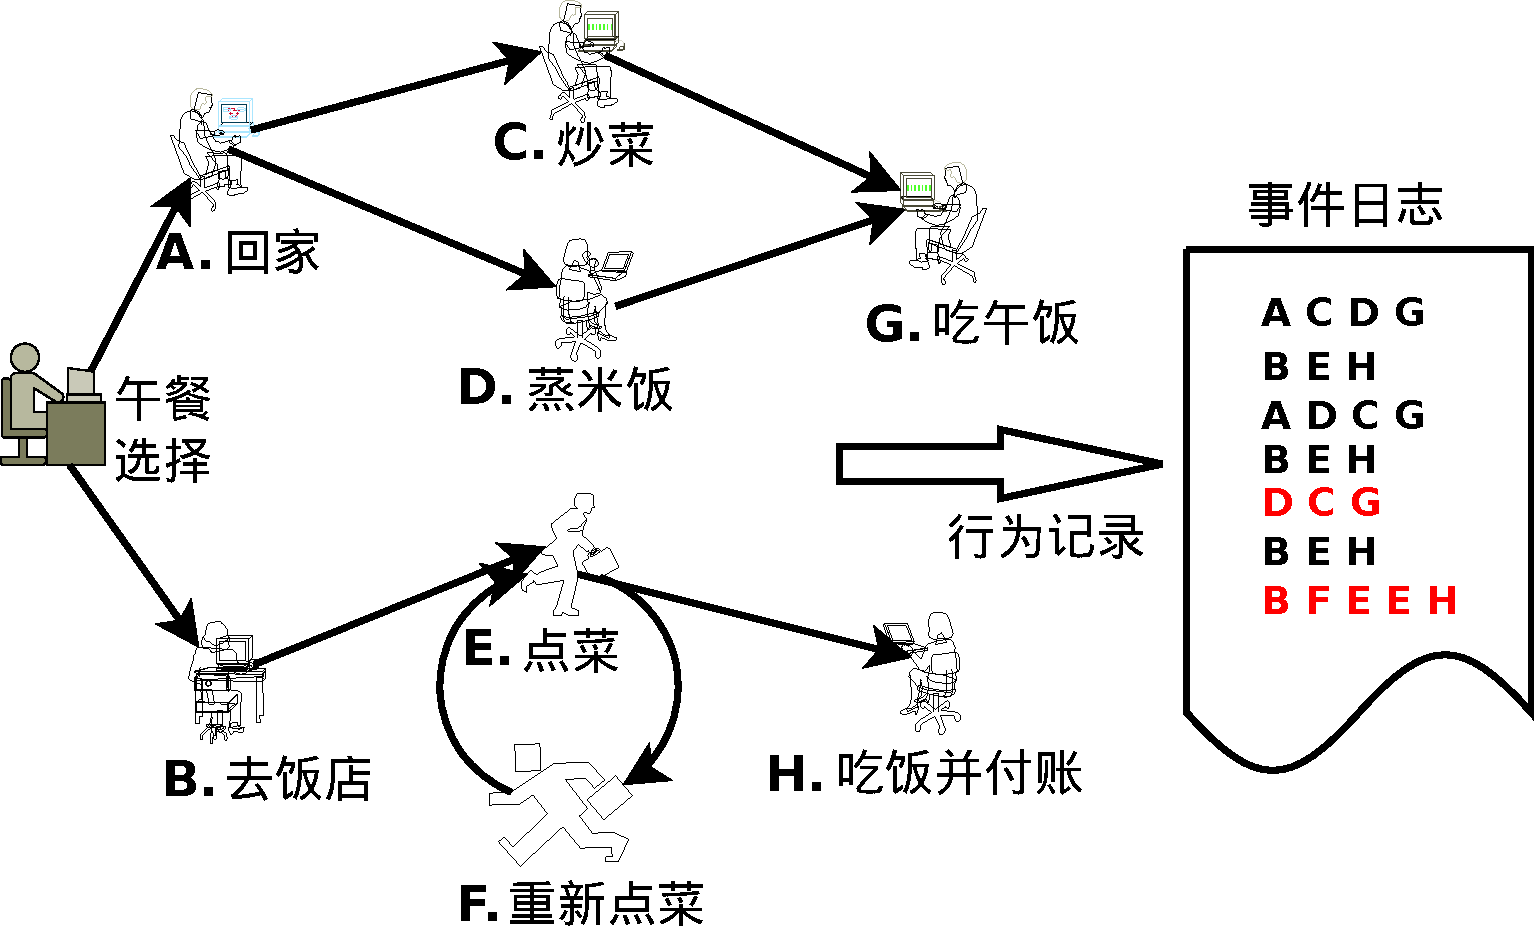
\includegraphics[width=0.7\textwidth]{lunchlog}
 \end{center}
\end{figure}
\note{业务过程与轨迹是业务过程管理领域的核心概概念。
	如图所示,一个业务过程就是一个由相互依赖的任务构成的网络,
	业务过程的一次执行产生一个轨迹,一条轨迹简单说就是一个由任务名称组成的字符串,
	多条轨迹记录下来就是日志。
%	说明业务过程是一个任务网络,业务过程执行一次就产生一轨迹,轨迹就是一个任务序列。
%日志是由轨迹组成的包,包中同一条轨迹可以出现多次。因为噪声的存在,导致轨迹跟真实发现的任务
%序列不一致,即产生污损轨迹。\\
%吃午饭这个例子,包含两个场景,回家自己做着吃,与吃饭店;回家吃饭,首先要回家,然后可以并行地蒸米饭与炒菜,最后吃饭;吃饭店则首先要去饭店,然后点菜,如果点的菜没有了,要重新点菜,最后吃饭付款。\\
%每次午饭,都有一条轨迹记录,如右边
%的日志,由于噪声,有些轨迹受到污损,如红色轨迹所示,回家的任务漏记了;以及点菜与再次点任务颠倒了\\
0.5分钟}
\end{frame}
%\begin{frame}{业务过程管理(Business Process Management,BPM)}
%	\begin{itemize}
%	\item 业务过程管理为业务过程及相关资源的设计、部署与分析等提供方法、技术、软件等工具。
%	\item 业务过程管理的实施,一般都有离不开某种过程感知的信息系统(PAIS)的支撑
%	\item 过程挖掘是BPM中一项重要研究课题。
%	\end{itemize}
%\begin{figure}
% \begin{center}
% \includegraphics[width=0.8\textwidth]{bpmlifecycle}
% \end{center}
%\end{figure}
%\end{frame}
\setfoot{1控制流}
\begin{frame}{过程挖掘}
	\begin{itemize}
	\item 基于业务过程运行的真实情况记录(日志)挖掘相关的知识
	\item 在实施过程中,过程建模占用$60\%\sim 80\%$的时间\tfn{J. Herbst, D. Karagiannis. Integrating Machine Learning and Workflow Management to
 Support Acquisition and Adaptation of Workflow Models. International Journal of Intelligent
  Systems in Accounting, Finance and Management, 2000, 9:67–92}。%\cite{herbstacc}
	\end{itemize}
\begin{figure}
 \begin{center}
 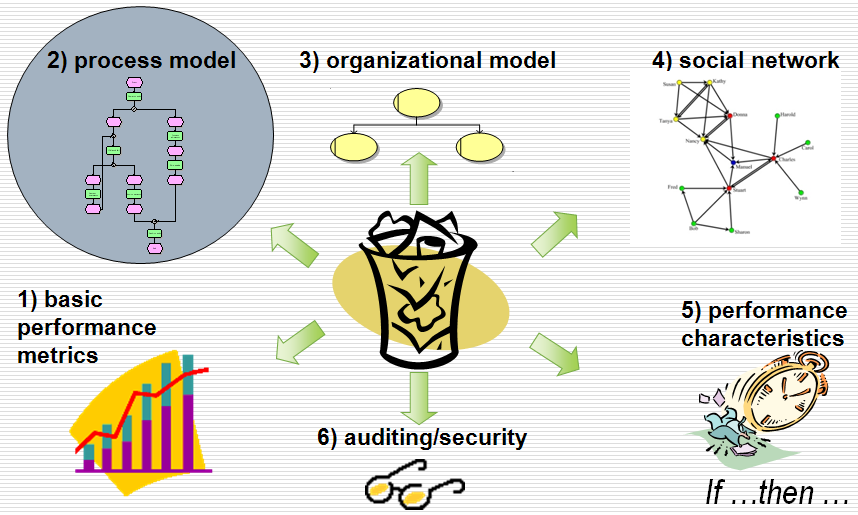
\includegraphics[width=0.9\textwidth]{pmfunctions}
 \end{center}
\end{figure}
\note{过程挖掘是业务过程领域的研究热点。
	所谓过程挖掘,就是从事件日志中挖掘有用的知识。
	包括挖掘性能因素、控制流挖掘、组织架构等等。
	由于具体的实施过程中,过程建模占用太多的时间,所以我们重点关注过程控制流的挖掘。
	%在点明过程挖掘是从日志中挖掘知识,读出其六大功能,说明建模比较费劲,强调我们关注控制流挖掘。\\
0.5分钟}
\end{frame}
\setfoot{1.5}
\begin{frame}{控制流挖掘}
	\begin{itemize}
	\item 从事件日志数据中,挖掘出一个合理的业务过程模型。
	\end{itemize}
\begin{figure}
 \begin{center}
 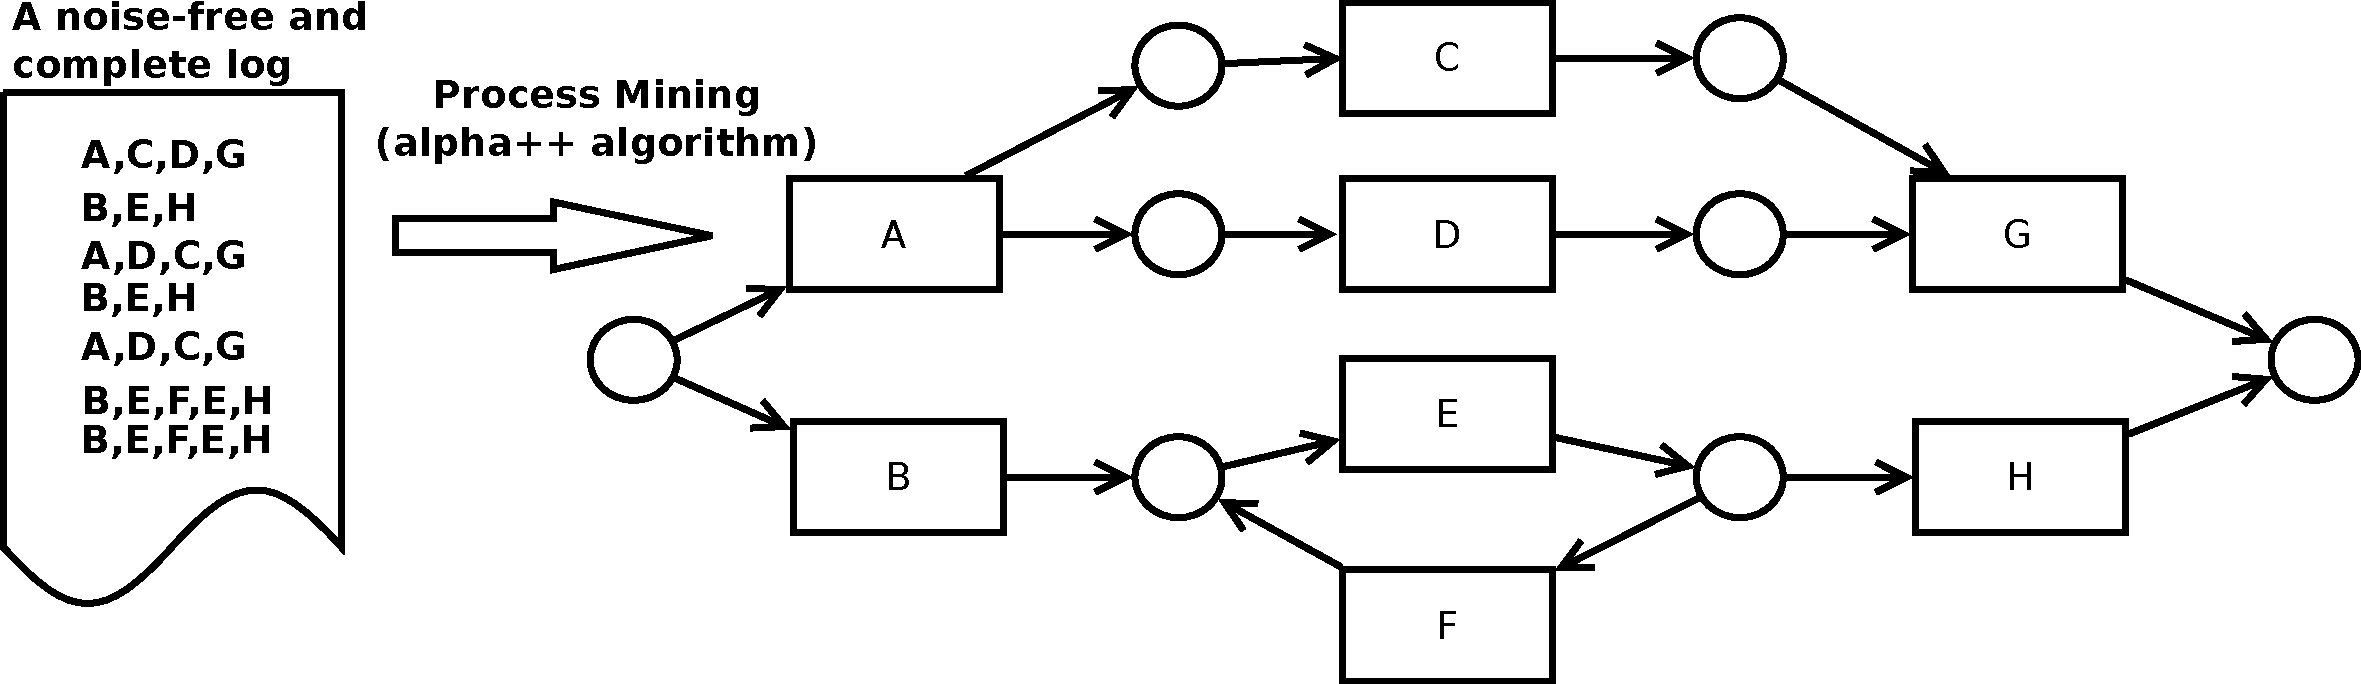
\includegraphics[width=1.0\textwidth]{processmining}
 \end{center}
\end{figure}
\begin{itemize}
	\item 挖掘结果质量依赖于
		\begin{itemize}
			\item 所用算法
			\item 数据(日志)质量
		\end{itemize}
\end{itemize}
\note{如图所示,所谓控制流挖掘就是从日志中挖掘出合理的流程模型。
	%强调模型挖掘要挖掘出合理的过程模型,或者说是任务有向图的结构信息,此处日志是前面所示吃午饭的事件日志,强调它未受噪声影响且局部信息完备,利用alpha++算法可以准确地得到午饭过程的控制模型。
	一般说来,挖掘结果的质量,一方向受限于挖掘算法的能力,另一方面取决于日志数据的质量。\\
0.5分钟}
\end{frame}



%%%%%%%%%%%%%%%%%%%%%%%%%%%%%%%%%%%%%%%%%%%%%%%%%%%%%%%%%%%%%%%%%%%%%%%%%%%%%%
%%---------------------------------------------------------------------------------------------------
%%---------------------------------------------------------------------------------------------------
%%---------------------------------------------------------------------------------------------------
%%===================================================================================================
%\section*{参考文献}
%%---------------------------------------------------------------------------------------------------
\begin{frame}\frametitle{参考文献}
\footnotesize
\bibliographystyle{splncs}
\bibliography{/home/hedong/Desktop/DOING/latestbib/lit}
%\begin{thebibliography}{10}
%{\beamertemplatebookbibitems
%
%\bibitem{zhangwenxiu}
%张文修, 吴伟志, 梁吉业, 李德玉.
%\newblock {\em 粗糙集理论与方法}.
%\newblock 科学出版社, 北京, 2001.}
%
%\bibitem{pawlak82}
%Z. Pawlak.
%\newblock Rough sets.
%\newblock {\em International Journal of Computer Information Science},
%  5:341--356, 1982.
%
%\bibitem{VariablePrecision}
%W.~Ziarko.
%\newblock Variable precision rough set model.
%\newblock {\em Journal of Computer and System Sciences}, 46:39--59, 1993.
%
%\bibitem{Katzberg1996ExtensionOfVPRS}
%J.~D. Katzberg and W.~Ziarko.
%\newblock Variable precision extension of rough sets.
%\newblock {\em Fundamenta Informaticae}, 27:155--168, 1996.
%
%\end{thebibliography}
%
\end{frame}


%%%%%%%%%%%%%%%%%%%%%%%%%%%%%%%%%%%%%%%%%%%%%%%%%%%%%%%%%%%%%%%%%%%%%%%%%%%%%%%%%%%%%%%%%%%%%%%
\setbeamertemplate{background canvas}[vertical shading][bottom=white,top=structure.fg!25]
\begin{frame}
 \begin{center}
{\huge \emph{\textcolor[rgb]{0.50,0.00,1.00}{Thank  ~you!}}}\\
\vspace{5mm}\large
%\begin{tabular}{ll}
%{\sc Author}:  & \textsf{Hedong ~ Yang}\\
%{\sc Address}: & Institute of Information System \& Engineering\\
%               & School of Software\\
%               & Tsinghua University, Beijing, China\\
%{\sc Post~code}:  & 100084\\
%%  {\sc Phone}:& +86--10--62773417\\
%%              & 13911204496\\
%  {\sc Email}: & \href{mailto:yanghd06@mails.tsinghua.edu.cn}{\color{blue}yanghd06@mails.tsinghua.edu.cn}\\
%\end{tabular}
\end{center}
\end{frame}

%%%%%%%%%%%%%%%%%%%%%%%%%%%%%%%%%%%%%%%%%%%%%%%%%%%%%%%%%%%%%%%%%%%%%%%%%%%%%%%%%%%%%%%%%%%%%%
\ifxetex
\else
\end{CJK}
\fi

%  \end{CJK*}
\end{document}

